\documentclass[border=8pt]{standalone}
\usepackage[T1]{fontenc}\usepackage[utf8]{inputenc}
\usepackage{helvet}\renewcommand{\familydefault}{\sfdefault}
\usepackage{tikz,xcolor}
\usetikzlibrary{arrows.meta,positioning,shapes.geometric,shapes.multipart,calc,fit,backgrounds,decorations.markings}
\definecolor{ink}{HTML}{1E1B16}\definecolor{paper}{HTML}{FBF8F2}\definecolor{clay}{HTML}{B5482A}\definecolor{soft}{HTML}{F1E9DA}\definecolor{pine}{HTML}{24402F}
\tikzset{
  every node/.style={font=\small,text=ink},
  >=Stealth, line/.style={draw=ink,line width=0.8pt},
  cls/.style={rectangle split,rectangle split parts=3,draw=ink,line width=0.8pt,fill=soft,align=left,inner xsep=6pt,inner ysep=4pt,
              rectangle split part align={center,left,left},minimum width=3.0cm},
  cls2/.style={rectangle split,rectangle split parts=2,draw=ink,line width=0.8pt,fill=soft,align=left,inner xsep=6pt,inner ysep=4pt,
              rectangle split part align={center,left},minimum width=3.0cm},
  box/.style={rectangle,draw=ink,line width=0.8pt,fill=soft,align=center,inner sep=5pt,minimum height=0.8cm},
  state/.style={rectangle,rounded corners=8pt,draw=ink,line width=0.8pt,fill=soft,align=center,inner sep=6pt,minimum width=2.2cm,minimum height=0.9cm},
  act/.style={rectangle,rounded corners=10pt,draw=ink,line width=0.8pt,fill=soft,align=center,inner sep=5pt,minimum width=2.4cm,minimum height=0.8cm},
  dec/.style={diamond,draw=ink,line width=0.8pt,fill=soft,inner sep=1pt,minimum width=0.9cm,minimum height=0.9cm},
  uc/.style={ellipse,draw=ink,line width=0.8pt,fill=soft,align=center,inner sep=3pt,minimum width=3.2cm,minimum height=1.0cm},
  note/.style={rectangle,draw=ink,line width=0.6pt,fill=yellow!12,align=left,inner sep=4pt,font=\footnotesize},
  lab/.style={font=\footnotesize,fill=paper,inner sep=1.5pt},
  err/.style={},
}
\newcommand{\actor}[3]{% x,y,label
  \draw[line width=0.8pt] (#1,#2+0.55) circle (0.17);
  \draw[line width=0.8pt] (#1,#2+0.38)--(#1,#2-0.15) (#1-0.3,#2+0.22)--(#1+0.3,#2+0.22) (#1,#2-0.15)--(#1-0.25,#2-0.6) (#1,#2-0.15)--(#1+0.25,#2-0.6);
  \node[font=\small] at (#1,#2-0.9) {#3};}
\begin{document}
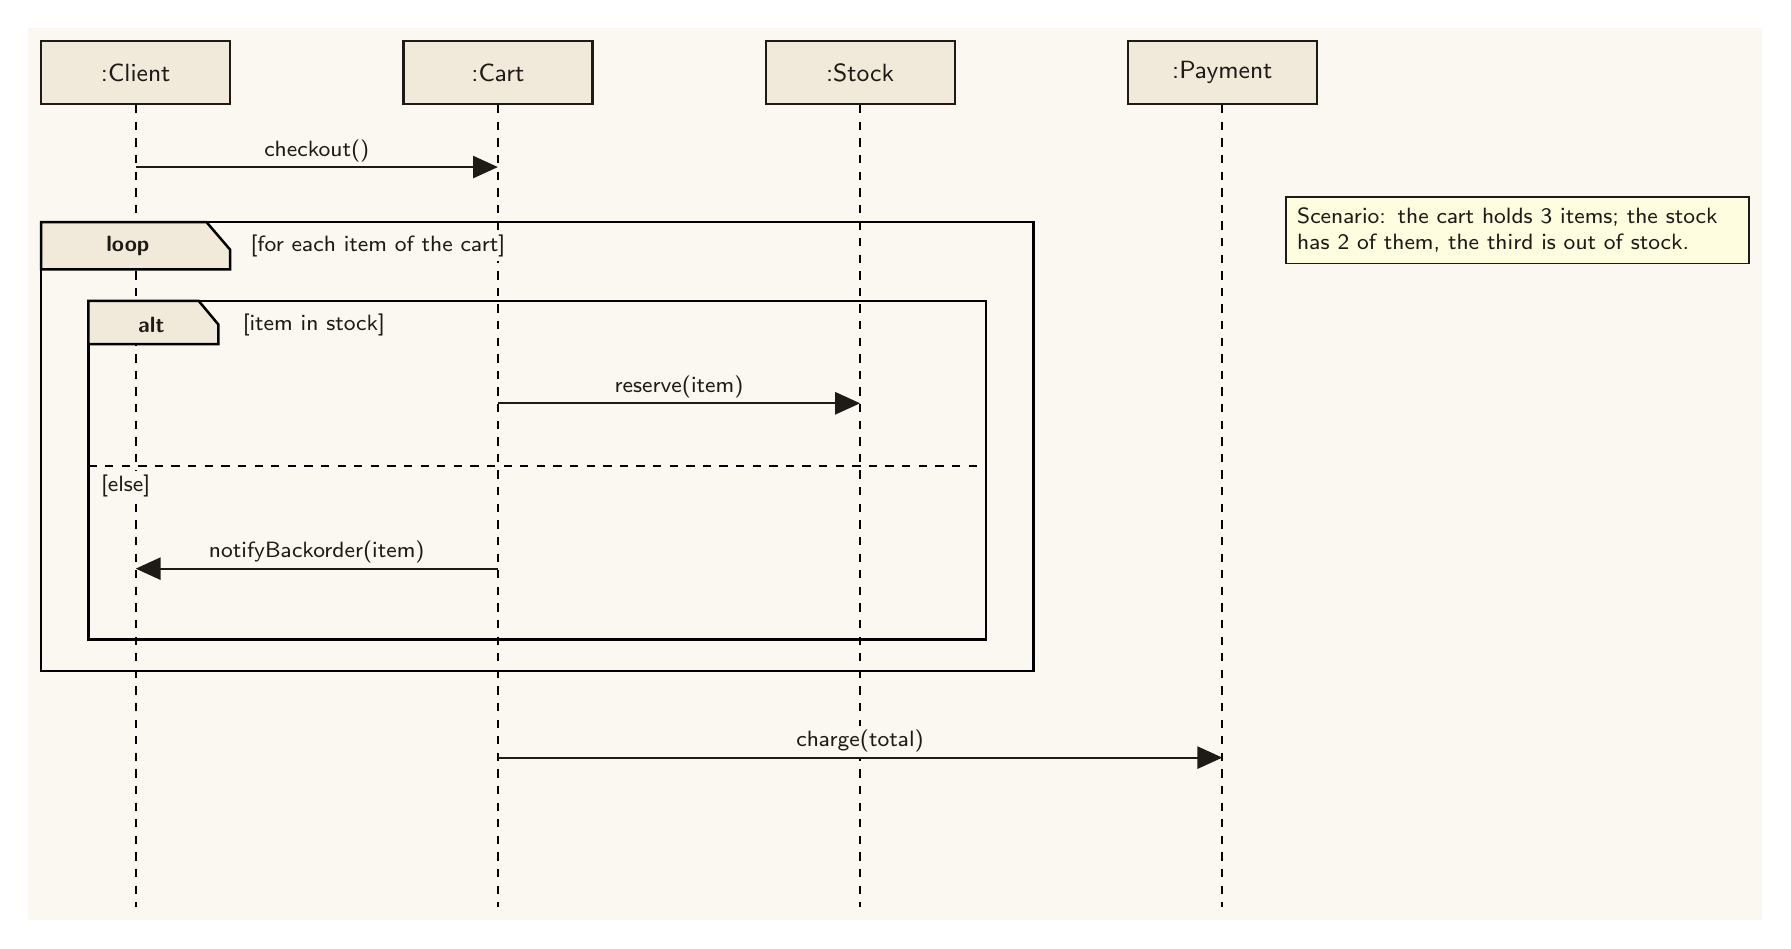
\begin{tikzpicture}[background rectangle/.style={fill=paper},show background rectangle]
\node[box,minimum width=2.4cm] (c) at (0,0) {:Client};
\node[box,minimum width=2.4cm] (k) at (4.6,0) {:Cart};
\node[box,minimum width=2.4cm] (s) at (9.2,0) {:Stock};
\node[box,minimum width=2.4cm] (p) at (13.8,0) {:Payment};
\draw[dashed,line width=0.7pt] (c.south)--(c.south |- 0,-10.6);
\draw[dashed,line width=0.7pt] (k.south)--(k.south |- 0,-10.6);
\draw[dashed,line width=0.7pt] (s.south)--(s.south |- 0,-10.6);
\draw[dashed,line width=0.7pt] (p.south)--(p.south |- 0,-10.6);
\draw[line,-{Triangle[length=9pt,width=8pt]}] (0,-1.2)--(4.6,-1.2) node[midway,above,lab]{checkout()};
\draw[line width=0.9pt] (-1.2,-1.9) rectangle (11.4,-7.6);
\draw[line width=0.9pt,fill=soft] (-1.2,-1.9)--(0.9,-1.9)--(1.2,-2.25)--(1.2,-2.5)--(-1.2,-2.5)--cycle;\node[font=\footnotesize\bfseries] at (-0.1,-2.2) {loop};
\node[lab,anchor=west] at (1.4,-2.2) {[for each item of the cart]};
\draw[line width=0.9pt] (-0.6,-2.9) rectangle (10.8,-7.2);
\draw[line width=0.9pt,fill=soft] (-0.6,-2.9)--(0.8,-2.9)--(1.05,-3.2)--(1.05,-3.45)--(-0.6,-3.45)--cycle;\node[font=\footnotesize\bfseries] at (0.2,-3.2) {alt};
\node[lab,anchor=west] at (1.3,-3.2) {[item in stock]};
\draw[line,-{Triangle[length=9pt,width=8pt]}] (4.6,-4.2)--(9.2,-4.2) node[midway,above,lab]{reserve(item)};
\draw[dashed,line width=0.7pt] (-0.6,-5.0)--(10.8,-5.0);
\node[lab,anchor=west] at (-0.5,-5.25) {[else]};
\draw[line,-{Triangle[length=9pt,width=8pt]}] (4.6,-6.3)--(0,-6.3) node[midway,above,lab]{notifyBackorder(item)};
\draw[line,-{Triangle[length=9pt,width=8pt]}] (4.6,-8.7)--(13.8,-8.7) node[midway,above,lab]{charge(total)};
\node[note,anchor=west,text width=5.6cm] at (14.6,-2.0) {Scenario: the cart holds 3 items; the stock has 2 of them, the third is out of stock.};
\end{tikzpicture}
\end{document}
